% !TEX encoding = UTF-8 Unicode
% !BIB TS-program = biber 
% !BIB program = biber    

% This file is MIT-Thesis.tex, a LaTeX template for formatting an MIT thesis with the mitthesis class.
%
% Version: 1.11, 2023/11/02
%
% Author: John H. Lienhard, copyright 2023. Reuse under the MIT license: https://ctan.org/license/mit 

% Documentation is here: https://ctan.org/pkg/mitthesis

%% Don't modify the \DocumentMetadata command unless you know what it does. 
%% If this command throws an "undefined" error, your latex system is out of date: try commenting this command out.
\DocumentMetadata{ 
	pdfstandard = a-2b,
	pdfversion  = 1.7,
	lang		= en-US,
%	debug		= {xmp-export}, % uncomment to output a separate xmpi file showing the metadata
}
%%%%%%%%%%%%%%%%%%%%%%%%%%%%%%%%%%%%%%%

\documentclass{mitthesis} %,fontset=libertine, fontset=newtx-sans-text, fontset=heros-stix2, fontset=stix2
%
% option [twoside]		gives facing-page behavior for printing; omitting twoside will eliminate even-numbered blank pages.
% option [lineno]	 	provides line numbers, as for editing
% option [mydesign] 	loads packages for color, title and list formats, margins, or captions: edit mydesign.tex to change defaults.
% option [fontset] is a keyvalue which can be:
%					 	pdftex or unicode engines:  defaultfonts, libertine, lucida
%					 	pdftex only: 				fira-newtxsf, newtx, newtx-sans-text
%						unicode engines (luatex):	heros-stix2, stix2, termes, termes-stix2
%					 	if no key value is given, fonts default to CMR (pdftex) or LMR (unicode), i.e., "the LaTeX font".
%					 	You can edit the fontset files or you can write your own, myfonts.tex, and do [fontset=myfonts].
%						If you are using multiple languages, load the babel package in your fontset file, before the fonts.

%%%%%%%%% Packages used in sample chapters (not otherwise required) %%%%%%%

%% Package for code listing in Appendix A.
\usepackage{listings}%   documentation is here https://ctan.org/pkg/listings

%% Set chemical formulas nicely
\usepackage[version=4]{mhchem}%   documentation is here https://ctan.org/pkg/mhchem

%% Latin filler used in Chapter 1, with a test for package version date. https://ctan.org/pkg/lipsum
\usepackage{lipsum}
\IfPackageAtLeastTF{lipsum}{2021/09/20}{\setlipsum{auto-lang=false}}{}


%%%%%%%%%  Graphics path (to figure files)  %%%%%%%%%%%%%%%%%%%%%%%%%%%%%%%%

%% Can set graphicspath to point to specific directories containing figures (the current directory is searched automatically)
%% For instance, to search a subdirectory of the current directory called "figures" and a parallel directory called "art", set:

% \graphicspath{ {figures/} {../art/} }% For details see: https://latexref.xyz/dev/latex2e.html#g_t_005cgraphicspath


%%%%%%%%%  Representative set-up for biblatex  %%%%%%%%%%%%%%%%%%%%%%%%%%%%%

\usepackage[style=ieee,maxbibnames=10,sorting=none]{biblatex}% style=ext-numeric-comp,articlein=false,giveninits=true
	\DefineBibliographyStrings{english}{url= \textsc{url} ,  }% replaces default "[Online]. Available" by "URL"

\usepackage{ragged2e}
\usepackage{booktabs, makecell, tabularx}
\renewcommand\theadfont{\bfseries}
\renewcommand\theadgape{}
\newcolumntype{L}{>{\RaggedRight}X}
\usepackage{enumitem}
\usepackage{etoolbox}
\usepackage{placeins}
\AtBeginEnvironment{table}{%
\setlist[enumerate]{nosep, % <-- list setup used in all tables
                     topsep = 0pt,
                     partopsep = 0pt,
                     wide,
                     label=\alph*),
                     before = \vspace{-0.6\baselineskip},
                     }
                        }

\addbibresource{cpr.bib}%% <== change to YOUR bib file <= CHANGE
\nocite{*}

%% to avoid split urls and stretched white space, you can set the bibliography ragged-right:
%\appto{\bibsetup}{\raggedright}

% biblatex is very powerful, and you can customize most aspects the reference list and citations to suit your needs.
% documentation is here: https://ctan.org/pkg/biblatex


%%%%%%%%%%  Option to use natbib   %%%%%%%%%%%%%%%%%%%%%%%%%%%%%%%%%%%%%%%%%

%\RequirePackage[numbers,sort&compress]{natbib}
 
%%% add bibliography to table of contents
%\apptocmd{\bibliography}{\addcontentsline{toc}{chapter}{\protect\textbf{\bibname}}}{}{}

%%% You can use this to rename the bibliography section
%\renewcommand{\bibname}{References}

%%% Can adjust space between bibliography items (change 4pt to something else; don't drop last two lengths, they are stretchable "glue")
%\setlength\bibsep{4pt plus 1pt minus 1pt}


%%%%%%%%%%  Table related packages  %%%%%%%%%%%%%%%%%%%%%%%%%%%%%%%%%%%%%%%%

\usepackage{booktabs}% better quality tables, https://ctan.org/pkg/booktabs
\usepackage{array}%    additional options for table columns, https://ctan.org/pkg/array
\usepackage[symbol]{footmisc}
\usepackage{algpseudocode}
\usepackage[linesnumbered,titlenumbered,ruled,vlined,resetcount,algosection]{algorithm2e}
\usepackage[usenames,dvipsnames]{xcolor}
\usepackage{color}
\usepackage{blkarray}
\usepackage{nicematrix}
\usepackage{adjustbox}
\usepackage[flushleft]{threeparttable}
\usepackage{colortbl}
%\captionsetup{%
%   justification=raggedright,
%   labelfont=bf,
%  singlelinecheck=off
%}
\usepackage{tikz}
\usetikzlibrary{shapes,arrows.meta,calc,fit,shapes.multipart, 
 positioning, backgrounds}

%%%%%%%%%%%%%% Tensor Double Arrow %%%%%%%%%%%%%%
\DeclareFontFamily{OMS}{oasy}{\skewchar\font48 }
\DeclareFontShape{OMS}{oasy}{m}{n}{%
         <-5.5> oasy5     <5.5-6.5> oasy6
      <6.5-7.5> oasy7     <7.5-8.5> oasy8
      <8.5-9.5> oasy9     <9.5->  oasy10
      }{}
\DeclareFontShape{OMS}{oasy}{b}{n}{%
       <-6> oabsy5
      <6-8> oabsy7
      <8->  oabsy10
      }{}
\DeclareSymbolFont{oasy}{OMS}{oasy}{m}{n}
\SetSymbolFont{oasy}{bold}{OMS}{oasy}{b}{n}

\DeclareMathSymbol{\smallleftarrow}     {\mathrel}{oasy}{"20}
\DeclareMathSymbol{\smallrightarrow}    {\mathrel}{oasy}{"21}
\DeclareMathSymbol{\smallleftrightarrow}{\mathrel}{oasy}{"24}

\newcommand{\tensor}[1]{\overset{\scriptscriptstyle\smallleftrightarrow}{#1}}
%%%%%%%%%%%%%%%%%%%%%%%%%%%%%%%%%%%%%%%%%%%%%%%%%%%%%


%%%%%%%%%%  Option for "double spacing" %%%%%%%%%%%%%%%%%%%%%%%%%%%%%%%%%%%%

%% Back in the typewriter era, double spaced lines were convenient for editing with a pencil. 
%% In typography, the separation between lines is called "leading", and it is usually set in 
%% proportion to the font size (i.e., when the font is loaded).  If you really feel the need 
%% to change the line separation, the most attractive results will be obtained by changing the
%% leading in proportion to the the current font size, rather than just doubling the space.

%% The setspace package provides a tool for changing line separation. Use these two commands here:
%
% \usepackage{setspace}%  documentation at https://ctan.org/pkg/setspace
% \setstretch{1.1}% you can choose some other value for the stretch of space between lines
%
%% Use one or more of the these commands AFTER the frontmatter
%
% \onehalfspacing
% \doublespacing
% \singlespacing  % will turn these effects off (you can use these anywhere in the document)

%% The best result may be to stay with leading selected by the typographer who set up the font.


%%%%%%%%%%%  Metadata  %%%%%%%%%%%%%%%%%%%%%%%%%%%%%%%%%%%%%%%%%%%%%%%%%%%%%%%

% Most of the document metadata is created automatically. 
% The following items should be adjusted to match your work. <================= !!!!!!!!!!

\hypersetup{%
	pdfsubject={Template for writing MIT theses with the mitthesis class},
	% Change this to briefly state topic of your thesis 
% 
	pdfkeywords={The University of Texas at Austin},
	% Add keywords that will help search engines and libraries to find your work.
	% Includes the name[s] of the author[s] 
	% (If you have used \DocumentMetadata, at line 15, you can just put "\CopyrightAuthor," for the names.)
%
	pdfurl={},
	% If you have a url for the thesis, put it here. Otherwise delete this.
	% (MIT Libraries will put your thesis in DSPACE with a persistent url after you submit it.)
%	
	pdfcontactemail={},
	% You can put a [permanent] email address into the metadata, if you like.
	% Otherwise delete this.
%
	pdfauthortitle={},
	% If you have a title, you can include it here.
}

%%%%%%%%%%%%%%  End preamble %%%%%%%%%%%%%%%%%%%%%%%%%%%%%%%%%%%%%%%%%%%%%%%%%%%%%%%%%%%%%%%%%%%%%
%%%%%%%%%%%%%%%%%%%%%%%%%%%%%%%%%%%%%%%%%%%%%%%%%%%%%%%%%%%%%%%%%%%%%%%%%%%%%%%%%%%%%%%%%%%%%%%%%%

\begin{document}

%%% edit the following commands to match your thesis %%%%%%%%%%

\title{Constrained Pressure Residual Implementation In UTCOMP Reservoir Simulator}

% \Author{Author full name}{Author department}[Author's first PREVIOUS degree][Author's second PREVIOUS degree][...
% Note that third, fourth, fifth, and sixth arguments are optional [] and may be omitted

% note on names: most of the following names are made up; Silas Holman was a physics professor at MIT in the 19th century.

\Author{Ahmad Assadeq}{Hildebrand Department of Petroleum and Geosystems Engineering}

% Use once for each degree fulfilled by thesis
% For two degrees from one department, leave the department argument blank for the second degree {}.
% \Degree{Bachelor of Science in Physics}{Department of Physics}
% \Degree{Master of Science in Physics}{}
\Degree{Master Of Science In Petroleum Engineering}{The University of Texas at Austin}

% If there is more than one supervisor, use the \Supervisor command for each.
\Supervisor{Kamy Sepehrnoori }{Professor of Petroleum and Geosystems Engineering}

% Professor who formally accepts theses for your department (e.g., the Graduate Officer, Professor Sméagol,...)
% If more than one department, use more than once
% **If you need to reduce vertical space, put the acceptor title in the second argument and leave the third blank {}.**
\SuppressAcceptorError
% \Acceptor{Primus Castor}{Professor of Wetlands Engineering}{Undergraduate Officer, Department of Physics}

% Usage: \DegreeDate{Month}{year}
% Valid degree months are September, February, or June
\SuppressMonthError
\DegreeDate{December}{2024}

% Date that final thesis is submitted to department
\ThesisDate{December 7, 2024}

%%%%%%  Choose whether to have a CREATIVE COMMONS License  %%%%%%%%%%%%%%%%%%%%%%%%%%%%%%%%%%%%%%
%
% If you are using a cc license, put details of your cc license here. 
% Omit this command if you are not using a cc license.
%
%\CClicense{CC BY-NC-ND 4.0}{https://creativecommons.org/licenses/by-nc-nd/4.0/}
%

%%%%%%%  Solutions for overflowing titlepage  %%%%%%%%%%%%%%%%%%%%%%%%%%%%%%%%%%%%%%%%%%%%%%%%%%%

% If your title page is overflowing (from too many names, degrees, etc.):
%
% (a) you can reduce the 12pt and 18pt skips between various blocks to 6pt with this command:
%
% \Tighten
%
% (b)  you can scale down the Signature block at the bottom with this command:
%
% \SignatureBlockSize{\small}  %or this one \SignatureBlockSize{\footnotesize}
%
% (c) you can put the acceptor name and title onto two lines, rather than three like this:
%
% \Acceptor{Tertius Castor}{Professor and Graduate Officer, Department of Research}{}
% \Acceptor{Quarta Castor}{Professor and Graduate Officer, Department of Mechanical Engineering}{}
%
% (d) you can change the font size of the the author name[s] with
%
%	\AuthorNameSize{\normalsize}
%
% (e) and you can omit any previous degrees from the title page, instead mentioning them in the Biosketch

% Also, if you prefer to keep the text toward the top of the page with most white space at the bottom, you
% can you this command to squash all of the vertical glue (stretchy space) with this command:
%
% \Squash 
%
% This command is useful when the text has not already reach the bottom of the page, since the glue gets squashed automatically
% when the page is too full.

%%%%%%%%%%%%%%%%%%%%%%%%%%%%%%%%%%%%%%%%%%%%%%%%%%%%%%%%%%%%%%%%%%%%%%%%%%%%%%%%%%%%%%%%%%%%%%%%%

%%% Make titlepage
\maketitle

%%%%%%%%% Contents that you need to write follows %%%%%%%%%%%%%%%%%%%%%%%%%%%%%%%%%%%%%%%%%%%%%%%%

% \includeonly{acknowledgments,biography,chapter1,chapter2,...,appendixa,...} 
%   for usage, see https://latexref.xyz/_005cinclude-_0026-_005cincludeonly.html

%%% Frontmatter (write this material in the mentioned files)  %%%%%%%%%%%%%%%%%%%%%%%%%%%%%%%%%%%%

% The abstract environment creates all the required headings and footers. 
% You only need to the text of the abstract in the file abstract.tex
\begin{abstract}
	% From mitthesis package
% Version: 1.01, 2023/06/19
% Documentation: https://ctan.org/pkg/mitthesis
%
% The abstract environment creates all the required headers and footnote. 
% You only need to add the text of the abstract itself.
%
% Approximately 500 words or less; try not to use formulas or special characters
% If you don't want an initial indentation, do \noindent at the start of the abstract

In the reservoir simulation community, the main focus of research related to \textit{Numerical Linear Algebra}, 
is to develop a physics-based preconditioner that can be efficiently coupled to a well-known high
performing Krylov-type iterative solver. This is due to the fact that the performance of these
solvers can significantly depend on the preconditioning of the matrix. Usually, preconditioning
is a mixture of experience, art and science and requires a domain specific knowledge of the problem
being solved. The industry-standard, state-of-the-art preconditioner is the Constrained Pressure Residual.
This report presents results related to the implementation of CPR on UTCOMP-RS\footnote{University Of Texas Compositional-Reservoir Simulator.}.
% use \input rather than \include because we're inside an environment
\end{abstract}

%\include{acknowledgments}% .tex extension is presumed by \include 

%\include{biography}% optional, see MIT Libraries https://libraries.mit.edu/distinctive-collections/thesis-specs/#format


%%% Table of contents and lists of stuff (delete lists you don't need, e.g., if no tables) %%%%%%%%

\tableofcontents
%\listoffigures
%\listoftables


%%% Chapters of thesis  %%%%%%%%%%%%%%%%%%%%%%%%%%%%%%%%%%%%%%%%%%%%%%%%%%%%%%%%%%%%%%%%%%%%%%%%%%%

%% If you want to use "double spacing", you should start here...

 % From mitthesis package
% Version: 1.04, 2023/10/19
% Documentation: https://ctan.org/pkg/mitthesis
\chapter{Introduction}
The use of models is part of our everyday life. In our modern society, we are sourounded by a myriad of complex systems that are
essential for the workings of our lifes from transportation, communication and food processing to energy production. Scientis and engineers
handle complexity by building simplified models that can be further enhanced to increase their ability to describe the complex systems.
In the petroleum industry, reservoir simulation is a branch of reservoir engineering that aims to develop models of the petroleum systems.
These models are built using knowledge of geological, geophysical and petrophysical properties of the petroleum reservoir system.
They are routinely used to describe fluid flow during the phase of field development planning and production, which enable the engineers 
to develop an optimum field production plan. The importance of reservoir simulation stems from the complexity of the physical systems that reservoir 
engineers attempt to describe. The use of mathematical models is essential to provide precise and valuable answers to the questions the simulator is 
set to answer. 

\begin{figure}[htb]
\centering
\resizebox{15cm}{!}{\pgfdeclarelayer{behind}
\pgfdeclarelayer{background}
\pgfdeclarelayer{foreground}
\pgfsetlayers{behind,background,main,foreground}
\tikzset{box/.style={draw, rectangle, rounded corners, thick, node 
 distance=7em, 
text width=6em, text centered, minimum height=3.5em}}
\tikzset{every node/.append style={font=\scriptsize}}

%************************************************************
%************************************************************
%  Define block styles
%************************************************************
%************************************************************
\tikzset{block/.style={rectangle split, draw, rectangle split parts=2,
text width=14em, text centered, rounded corners, minimum height=4em},
grnblock/.style={rectangle, draw, fill=green!20, text width=10em, text 
centered, rounded corners, minimum height=4em}, 
whtblock/.style={rectangle, draw, fill=white!20, text width=10em, text 
centered, minimum height=3em},    
ylwblock/.style={rectangle, draw, fill=yellow, text width=10em, text 
centered, minimum height=3em}, 
line/.style={draw, -{Latex[length=2mm,width=1mm]}},
cloud/.style={draw, ellipse,fill=white!20, node distance=3cm,minimum height=3em},  
container1/.style={draw, rectangle,dashed,inner sep=0.28cm, rounded
corners,fill=green!8,minimum height=2.4cm,minimum width=5.6cm},
container2/.style={draw, rectangle,dashed,inner sep=0.28cm, rounded
corners,fill=red!8,minimum height=4.cm,minimum width=6.3cm},
container3/.style={draw, rectangle,dashed,inner sep=0.28cm, rounded
corners,fill=gray!15,minimum height=3cm,minimum width=6.3cm},
arrow/.style={-, thick}
}
%************************************************************
%************************************************************ 
\begin{tikzpicture}[node distance = 1.20cm, auto]
%************************************************************
%************************************************************
%  Draw nodes
%************************************************************
\node [whtblock,font=\fontsize{10}{0}\selectfont] (resgrid) {Reservoir geometrical representation: grid data points.};
%===============================================    
%  Constituent elastic parameters
%===============================================  
\node [block, below=of resgrid,rectangle split part fill= 
{orange!20,blue!3},font=\fontsize{10}{0}\selectfont, yshift=1cm] (petro) 
{\textbf{Petrophysical Parameters}
\nodepart[text width=3cm]{two} 	$\phi,\ \boldmath{\tensor{K}},\ \Delta x,\ \Delta y,\ \Delta z$\\
				$P_{c}(S_{w}),\ K_{rw},\ K_{ro},\ K_{rg}$};
% ****************************************************
% ****************************************************
 \node [right=3.9cm of resgrid, yshift=1.2cm] [fill=white,draw,font=\fontsize{12}{0}\selectfont] 
 (flowmodel) {\textbf{Flow Model}};

 \node [below=2.7cm of resgrid, xshift=4.5cm] [fill=white,draw,font=\fontsize{12}{0}\selectfont] 
 (wellmodel) {\textbf{Well Model}};

\node [below=of wellmodel, yshift=0cm,block,anchor=center,rectangle split part fill= {orange!20,blue!3},font=\fontsize{10}{0}\selectfont] (welleq) 
{\textbf{Well Model Equations}
\nodepart[text width=5cm] 
{two}$q_{\alpha,i} = J_{i}\lambda_{\alpha,i}(p_{i} - p_{bhp} - H_{wi})$\\
$J = \frac{\theta K h}{\ln{r_{e}/r_{w}}+S}$\\
[1em] 
}; 

\node [below=of flowmodel, yshift=-0.5cm,block,anchor=center,rectangle split part fill= {orange!20,blue!3},font=\fontsize{10}{0}\selectfont] (MatParm) 
{\textbf{Mathematical Model Of Flow (PDE)}
\nodepart[text width=5cm] 
{two}$\partial_{t}(\phi b_{w}S_{w}) + \nabla \cdot (b_{w}\vec{u_{w}}) = b_{w}q_{w}$\\
$\partial_{t}(\phi b_{o}S_{o}) + \nabla \cdot (b_{o}\vec{u_{o}}) = b_{o}q_{o}$\\
$\partial_{t}\phi[b_{g}S_{g}+b_{o}R_{s}S_{o}] + \nabla \cdot (b_{g}\vec{u_{g}} + b_{o}R_{s}\vec{u_{o}}) = b_{g}q_{g} + b_{o}R_{s}q_{o}$\\
[1em] 
}; 

\begin{pgfonlayer}{background}
 \coordinate (aux1) at ([yshift=3mm]resgrid.north);
 \node [container1,fit=(aux1)(petro)] (cont3) 
 {};
   \node at (cont3.north) [fill=white,draw,font=\fontsize{12}{0}\selectfont] 
 {\textbf{Geological Properties}};
 %-----------------------------------------------------------
\end{pgfonlayer}

\begin{pgfonlayer}{behind}
 \coordinate (aux2) at ([yshift=-8mm, xshift=5.3cm]resgrid.east);
 \node[container2, fit=(aux2)] (cont1) 
 {};
\end{pgfonlayer}

\begin{pgfonlayer}{behind}
 \coordinate (aux2) at ([yshift=-15mm, xshift=-3cm]cont1.south);
 \node[container3, fit=(aux2), yshift=-0.8cm] (cont2) 
 {};
%\draw[color=red] (cont1.south) to (cont2.east);
\draw[arrow](cont1.south)+(1, 0) -- ++(1,-1) |- (cont2.east);
\draw[arrow](cont3.south)+(-1, 0) -- ++(-1,-1) |- (cont2.west);
\draw[arrow](cont3.east)+(0,0.04) -- (cont1.west);
\end{pgfonlayer}
\end{tikzpicture}
}
\caption{Models used in a reservoir simulator.}\label{models}
\end{figure}

There are several physical systems within a petroleum reservoir that a reservoir simulator needs to model. 
These can include the grid dimensions representing the reservoir and the geological properties of the reservoir such as porosity, 
permeability and multiphase fluid flow parameters like capillary pressure and relative permeability. A fluid flow model that consists of 
conservation laws and a constitutive Darcy's law for flow in porous media must also be incorporated as a model to the reservoir simulator.
Several fluid modeling techniques are used in the industry, the most commonly known are the \textit{Black-oil} and \textit{Compositional} models.
Moreover, the boundary conditions for the differential equations describing the fluid flow are the wells, both injectors and producers. 
The wells are also routinely modeled in the simulator using differential equations to describe inflow performance of the wells. One of well models
main objectives is to relate the reservoir gridblock pressure to the well bottom hole pressure. More sophisticated well models handle cross flow and
multilateral, horizontal and slanted wells. Reservoir simulators can also include additional models to simulate networks of fractures, surface facilities,
enhanced oil recovery and geomechanics. The main standard models that a simple reservoir simulator must incorporate are summarized in figure \ref{models}.

The inner components of reservoir simulators are more or less universal. Each simulator has to support a 
gridding infrastructure to support discretization of the simulation domain, a nonlinear solver (usually based on Newton's Method) to 
solve the nonlinear coupled PDEs of fluid flow, a linear solver that will solve the matrix produced by the nonlinear solver, a timestepping
mechanism guided by some convergence criteria of the nonlinear solver and an I/O system to generate results requested by the user for post-processing.

At the \textit{Center for Subsurface Energy and the Environment}, there are three variants of reservoir simulators. The full-fledged compositional 
simulator \texttt{UTCOMPRS} is capable of handling up to four-phase flow, an aqueous, oleic, gaseous and an additional nonaqueous liquid phase. 
The simulator was originally developed in the 1990s\supercite{utcomp}. The second simulator \texttt{UTCHEMRS}, is specialized in chemical flooding.
\texttt{UTCOMPRS} and \texttt{UTCHEMRS} supports an Adaptive-Implicit formulation, with gridding supported by both Cartesian and the industry standard
Corner-Point Geometry. The third \texttt{Multi-Purpose Simulator (MPS)} is focused on performing parallel simulation for large complex reservoirs operating under
various recovery processes. The modeling group maintains the development of all three simulators. 

The overall algorithm of a reservoir simulator can be simplified by focusing on the essential components. These will be found in every reservoir simulator, whether
its foucsed on research or industrial activities. The simulation process is depicted in figure \ref{simulator}. The process commences by parsing the input files that describe the
reservoir and boundary conditions as specified by wells or aquifers. Then an algroithm to build the simulation grid is run and connectivity graph is constructed. Then the three main
loops of the simulator are entered. These loops consist of a time loop that will finish once the end of specified simulation time is reached. The second inner loop is Newtonian loop,
that will end once the set of nonlinear equations are solved with acceptable tolerance. The third inner loop is the linear solver loop that will finish once the linear system of equations
is solved with acceptable tolerance.

\begin{figure}[htb]
\raggedright
\resizebox{15cm}{!}{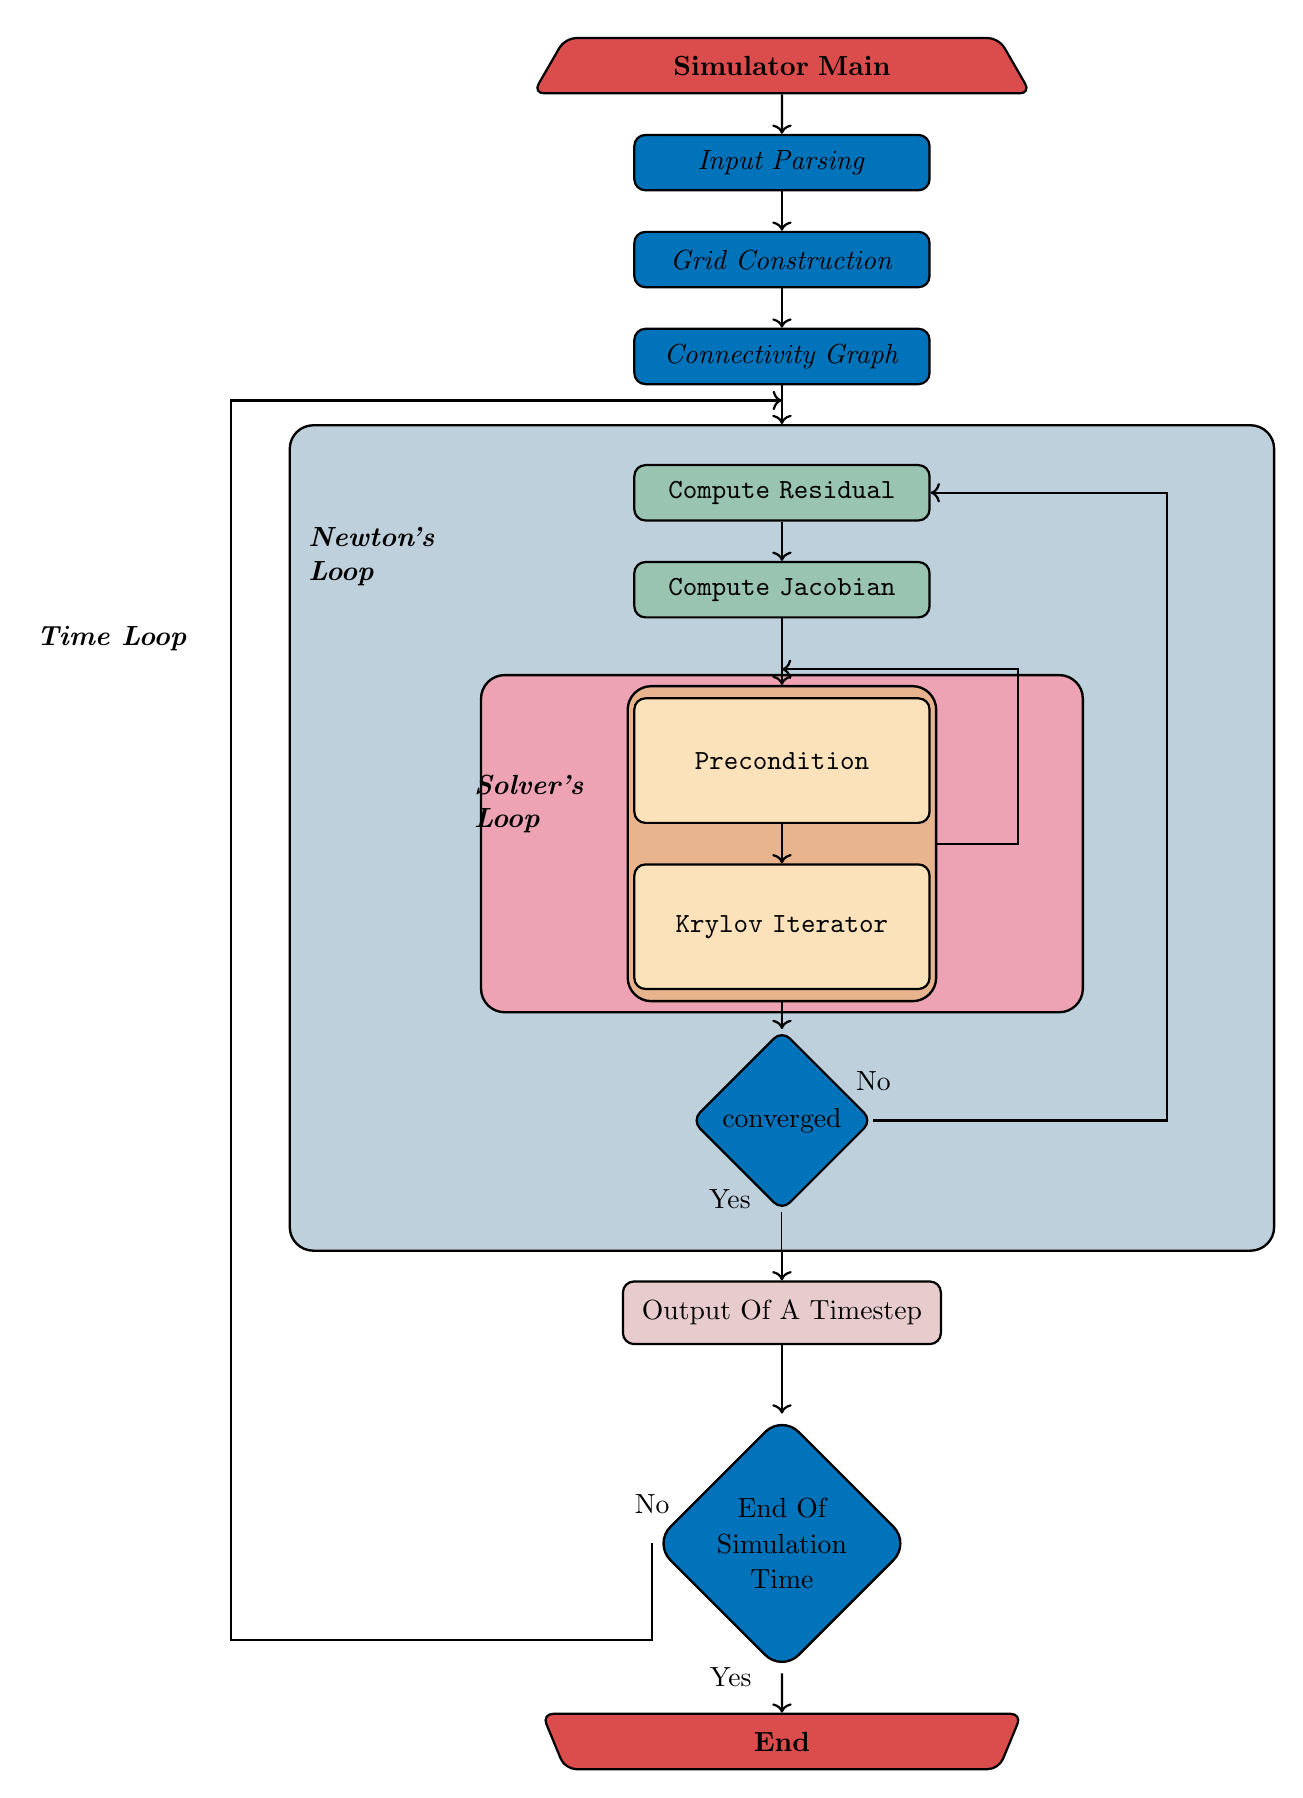
\begin{tikzpicture} [
output/.style    = { rectangle, draw=black, thick, 
    fill=embeddings_color,
    rounded corners, minimum height=2em },
post/.style    = { rectangle, draw=black, thick, 
    fill=emb_color, text width=4em, text centered,
    rounded corners, minimum height=2em },
addnorm/.style    = { rectangle, draw=black, thick, 
    fill=cadmgreen!40, text width=10em, text centered,
    rounded corners, minimum height=2em },
four/.style    = { rectangle, draw=black, thick, 
    fill=fourier_color, text width=10em, text centered,
    rounded corners, minimum height=4.5em },
grid/.style    = { rectangle, draw=black, thick, 
    fill=frenchblue, text width=10em, text centered,
    rounded corners, minimum height=2em },
conn/.style    = { rectangle, draw=black, thick, 
    fill=frenchblue, text width=10em, text centered,
    rounded corners, minimum height=2em },
main/.style    = { trapezium, draw=black, thick, 
    fill=boston!70, text width=10em, text centered,
    rounded corners, minimum height=2em },
end/.style    = { trapezium , trapezium angle=-67.5, draw=black, thick, 
    fill=boston!70, text width=10em, text centered,
    rounded corners, minimum height=2em },
input/.style    = { rectangle, draw=black, thick, 
    fill=frenchblue, text width=10em, text centered,
    rounded corners, minimum height=2em },
conv/.style    = { diamond, draw=black, thick, 
    fill=frenchblue, text centered,
    rounded corners},
line/.style     = { draw, thick, <-, shorten >=0pt },
]
\definecolor{emb_color}{RGB}{252,224,225}
\definecolor{embeddings_color}{RGB}{232,204,205}
\definecolor{cadmgreen}{rgb}{0.0, 0.42, 0.24}
\definecolor{chocolate}{RGB}{210,105,30}
\definecolor{alizarin}{rgb}{0.82, 0.1, 0.26}
\definecolor{airforceblue}{rgb}{0.36, 0.54, 0.66}
\definecolor{boston}{rgb}{0.8, 0.0, 0.0}
\definecolor{frenchblue}{rgb}{0.0, 0.45, 0.73}
\definecolor{fourier_color}{RGB}{252,226,187}
% Define nodes in a matrix
\matrix [column sep=1mm, row sep=5mm] {
    & \node [main] (main) {\textbf{Simulator Main}};         & \\
    & \node [input] (input) {\textit{Input Parsing}};  & \\
    & \node [grid] (grid) {\textit{Grid Construction}};                     & \\
    & \node [conn] (connect) {\textit{Connectivity Graph}};                     & \\\\
    & \node [addnorm] (res) {\texttt{Compute Residual}};       & \\
    & \node [addnorm] (jac) {\texttt{Compute Jacobian}};       & \\
    & \coordinate (null2);                                & \\
	& \node [four] (cpr) {\texttt{Precondition}};        & \\
	& \node [four] (krylov) {\texttt{Krylov Iterator}};                & \\
    & \node [conv] (conv1) {converged};                & \\
    & \coordinate (null1);                                & \\
};

\node[below = 1cm of conv1] (output) {Output Of A Timestep};
\node[conv, below = 1cm of output, line width=0.03cm,draw, rounded corners=0.3cm,] (conv2) {\shortstack{End Of \\\\Simulation \\ \\Time}};
\node [yshift=0.5cm]at (conv2.west) {No};
\node [xshift=1cm, yshift=-1.7cm]at (conv2.west) {Yes};

\begin{pgfonlayer}{background}
    \node[fit=(output),output](post){};
    \coordinate (N1) at (post.west|-krylov);
    \coordinate (N2) at (post.east|-krylov);
    \node[inner xsep=120pt,inner ysep=14pt,fit=(res)(krylov)(N1)(N2)(conv1),fill=airforceblue!40, line width=0.03cm,draw, rounded corners=0.3cm,label={[align=left, xshift=-8.5cm,yshift=-3cm]\textbf{\textit{Time Loop}}}](timeloop){};
    \node[inner xsep=55pt,inner ysep=8pt,fit=(cpr)(krylov),fill=alizarin!40, line width=0.03cm,draw, rounded corners=0.3cm,label={[align=left,xshift=-5.2cm,yshift=1cm]\textbf{\textit{Newton's}} \\\textit{\textbf{Loop}}}](newton){};
    \node[inner xsep=2pt,inner ysep=4pt,fit=(cpr)(krylov),fill=chocolate!50, line width=0.03cm,draw, rounded corners=0.3cm,label={[align=left,xshift=-3.2cm,yshift=-2cm]\textit{\textbf{Solver's}} \\\textit{\textbf{Loop}}}](solver){};
    \node [yshift=0.5cm]at (conv1.east) {No};
    \node [xshift=0.5cm, yshift=-1cm]at (conv1.west) {Yes};
\end{pgfonlayer}

\node[end, below= 5mm of conv2](end){\textbf{End}};

% connect all nodes defined above
\begin{scope} [every path/.style=line]
\path (input)       --  (main);
\path (grid)       --  (input);
\path (connect)       --  (grid);
\path (timeloop)        --  (connect);
\path (jac)          --  (res);
\path (solver)          --  (jac);
\path (solver.north)+(0,0.2)       --++  (3,0.2) |- (solver.east);
\path (krylov)     --  (cpr);
\path (post)  --  (timeloop) coordinate[midway](null1) ;
\path (timeloop.north)+(0,0.3)  --++  (-7,0.3) -- (-7,-12.65) -| (conv2.west);
\path  (conv1.north) -- (solver.south);
\path  (res.east)--++(3,0) |-(conv1.east);
\path (conv2) -- (post);
\path (end) -- (conv2);
\end{scope}
\path [draw] (timeloop.south)--(conv1);

\end{tikzpicture}
}
\caption{Generic Algorithm Of A Reservoir Simulator.}\label{simulator}
\end{figure}
\clearpage

A crucial advantage of simulation tools over classical engineering analysis practices is the ability
to perform a large number of calculations in an efficient way. In reservoir simulation, the most taxing
component of runing a simulator is usually the linear solver. Therefore, research in developing efficient
techniques in solving large system of equations is ample in the reservoir simulation literature. The main
focus is usually on developing scalable preconditioners that can be combined with iterative Krylov-based 
iterators. The industry standard preconditioner is the Constrained Pressure Residual. This preconditioner
has its roots in the works of Wallis\supercite{Wallis_1983,Wallis_1985}, the essential idea relies on decoupling
the resulting system of linear equations by isolating the elliptic dominant part of the system (pressure) from 
the hyperbolic (saturation or concentration) part of the system. 

The convergance of a Krylov iterative solver depends essentially on the preconditioner. The prototypical Krylov method, the
Conjugate Gradient can handle Symmetric-Positive-Definite matrices. For reservoir simulation cases, where matrices are ill-conditioned and
not symmetric, the Generalized Minimum Residual \textit{GMRES}, is used\supercite{roy}. 

\section{Spatial Discretization}
The discretization techniques consist an active area of research in numerical solution of PDEs. Historically reservoir simulators used 
finite-difference method to discretize the nonlinear PDE system. The current generation of reservoir simulators, both originating from
academy and industry, utilize the Two-Point Flux-Approximation (TPFA), which is based on a finite volume method. Finit-volume mehthods 
originate from a physically motivated conservation law. A more accurate method for high-resolution grids with non-orthogonal oriented 
grids with respect to the permeability tensor is the Multi-Point Flux-Approximation (MPFA) \cite{mpfa}. TPFA is not consistent for grids
that are not K-orthogonal and a more accurate discretization technique must be used. In this brief description the discussion will be
restricted the simple case of orthogonal grids and the TPFA will be discussed. 

The formulation used in \texttt{UTCOMPRS} can be described by the following system of PDEs\supercite{phdfernandes}:
\begingroup\makeatletter\def\f@size{12}\check@mathfonts
\begin{equation}
	\begin{cases}
		\frac{1}{V_{b}} \frac{\partial N_{k}}{\partial t} = \sum_{j=2}^{n_{p}}\Big\{\nabla \cdot\Big( x_{kj}\xi_{j}\frac{k_{rj}}{\mu_{j}}\tensor{K}\cdot\nabla\Phi_{j}\Big) + \nabla \cdot \Big(\phi S_{j}\xi_{j}\tensor{\Lambda}_{kj}\cdot\nabla x_{kj}\Big)\Big\} - \frac{q_{k}}{V_{b}}, \ k=1,...,n_{c}\\\\
		\frac{1}{V_{b}} \frac{\partial N_{w}}{\partial t} = \nabla \cdot \Big(\xi_{w}\frac{k_{rw}}{\mu_{w}}\tensor{K}\cdot \nabla\Phi_{w}\Big) - \frac{q_{w}}{V_{b}}
	\end{cases}
\end{equation}\endgroup

\begin{figure}[htb]
\raggedright
\resizebox{13cm}{!}{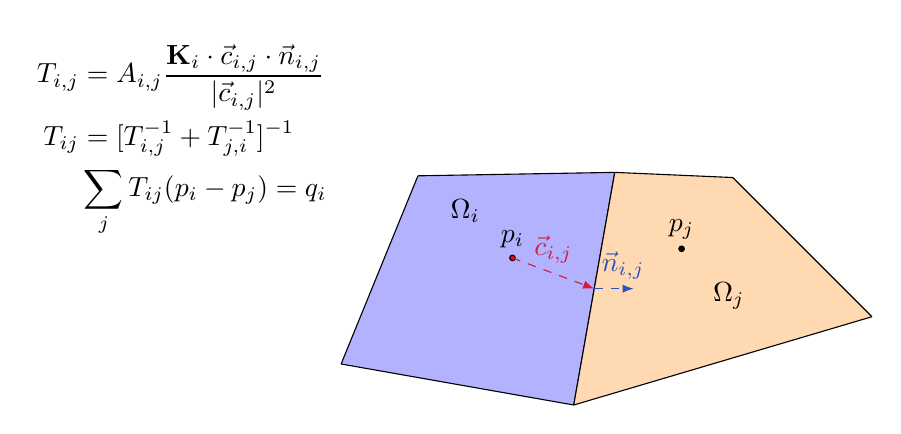
\begin{tikzpicture}
\colorlet{veccol}{green!45!black}
\colorlet{myred}{red!90!black}
\colorlet{myblue}{blue!90!black}
\colorlet{mypurple}{blue!50!red!80!black!80}
\tikzstyle{vector}=[->,very thick,veccol]
\usetikzlibrary{arrows.meta}
\tikzstyle{thin arrow}=[dashed,thin,-{Latex[length=4,width=3]}]
\definecolor{alizarin}{rgb}{0.82, 0.1, 0.26}
\definecolor{ceruleanblue}{rgb}{0.16, 0.32, 0.75}

 \path[fill=blue!30] (0,0) coordinate(p1) --  ++(1:2.5) coordinate(p2)
 -- ++(30:0) coordinate(p3) --
 ++(-100:3) coordinate(p4) --  ++(170:3) coordinate(p5);

 \coordinate (c1) at (barycentric cs:p1=1,p2=1,p3=1,p4=1,p5=1);
 \node at (c1) [xshift=-0.6cm, yshift=0.6cm] {$\Omega_{i}$};
 \draw[fill=red](c1) circle (1 pt) node  [above] {$p_{i}$};

 \foreach \X [count=\Y] in {2,...,6}
 {\ifnum\X=6
   \path (p\Y) -- (p1) coordinate[pos=0](a\Y) coordinate[pos=1](a1)
   coordinate[pos=0.5](m1);
   \draw (a\Y) -- (a1);
   %\draw[-latex] (m1) -- ($ (m1)!1.2cm!90:(p1) $) node[pos=1.2]{$a_{\Y}$};
  \else
   \path (p\Y) -- (p\X) coordinate[pos=0](a\Y) coordinate[pos=1](a\X)
   coordinate[pos=0.5](m\X);
   \draw (a\Y) -- (a\X);
   %\draw[-latex] (m\X) -- ($ (m\X)!1.2cm!90:(p\X) $) node[pos=1.2]{$a_{\Y}$};
  \fi}

 \path[fill=orange!30] (p3) coordinate(s1) --  ++(p1) coordinate(s2) -- ++(-2.5:1.5) coordinate(s3) 
 -- ++(-45:2.5) coordinate(s4) --
 (p4) coordinate(s5) ;

 \coordinate (c2) at (barycentric cs:s1=1,s2=1,s3=1,s4=1,s5=1);
 \node at (c2) [xshift=0.6cm, yshift=-0.6cm] {$\Omega_{j}$};
 \draw[fill=black](c2) circle (1 pt) node [above] {$p_{j}$};

 \foreach \X [count=\Y] in {2,...,6}
 {\ifnum\X=6
   \path (s\Y) -- (s1) coordinate[pos=0](b\Y) coordinate[pos=1](b1)
   coordinate[pos=0.5](t1);
   \draw (b\Y) -- (b1);
   %\draw[-latex] (m1) -- ($ (m1)!1.2cm!90:(p1) $) node[pos=1.2]{$a_{\Y}$};
  \else
   \path (s\Y) -- (s\X) coordinate[pos=0](b\Y) coordinate[pos=1](b\X)
   coordinate[pos=0.5](t\X);
   \draw (b\Y) -- (b\X);
   %\draw[-latex] (m\X) -- ($ (m\X)!1.2cm!90:(p\X) $) node[pos=1.2]{$a_{\Y}$};
  \fi}

  \coordinate (s1+s5) at ($0.5*(s1)+0.5*(s5)$);
  \draw[vector,thin arrow,alizarin] (barycentric cs:p1=1,p2=1,p3=1,p4=1,p5=1) -- (s1+s5) node[midway,above] {$\vec{\vb{c}}_{i,j}$};
  \draw[vector,thin arrow,ceruleanblue] (s1+s5) -- ++(0.5,0) coordinate(s1+s5) node[midway,above] {$ \ \ \vec{\vb{n}}_{i,j}$};

\node at (-3,0.5) {$\begin{aligned}
	T_{i,j} &= A_{i,j}\frac{\mathbf{\tensor{K}}_{i}\cdot\vec{c}_{i,j}\cdot\vec{n}_{i,j}}{|\vec{c}_{i,j}|^{2}}\\
		T_{ij}	&= [T_{i,j}^{-1}+T_{j,i}^{-1}]^{-1}\\
		&\sum_{j}T_{ij}(p_{i}-p_{j}) = q_{i}
		\end{aligned}$};

\end{tikzpicture}
}
\caption{Two-Point Flux-Approximation.}\label{tpfa}
\end{figure}



\section{Temporal Discretization}
The discretization of the time variable is of significant importance to the overall solution procedure.
Explicit and implicit methods are used to treat the time derivative. The implicit procedure produces the 
system of equations that needs to be solved, while the explicit technique results in a problem that can be
solved sequentially. The explicit method can compute the state of the system at time $n+1$ exclusively from 
variables evaluated at time level $n$. While the implicit method constructs an equation for variables at level
$n+1$ that involves both variables at level $n$ and $n+1$. Mathematically the two techniques can be represented by 
the following, if $Y(t)$ represents the state of the system at time $t$:
\begingroup\makeatletter\def\f@size{12}\check@mathfonts
\begin{equation}
	\begin{cases}
		Y(t+\Delta t) = F(Y(t)), \ \text{(Explicit scheme)}\\\\
		G(Y(t), Y(t+\Delta t)) = 0, \ \text{(Implicit scheme)}\\\\
		Y(t+\Delta t) = F(Y(t+\Delta t)) + G(Y(t)), \ \text{(Mixed scheme)}
	\end{cases}
\end{equation}\endgroup
The explicit methods are easier to implement, but their fallout is a severe restriction on timestep size, 
requiring a small timestep to converge. Implicit methods on the other hand, will result in large systems of 
equations that will take time to solve, but they allow for the selection of large timestep sizes resulting in 
overall outperformance to the explicit methods. In the reservoir simulation literature, there exists a variety of
different types of time discretization, with special emphasis on implicit and mixed (implicit on stiff variables and explicit on others) 
discretization techniques. In \texttt{UTCOMPRS}, extensive research was conducted to implement several formulations. Each formulation treats
different variables with different degrees of implicitness. A summary of the most important formulations is give in table \ref{formulations}.
Below an example of discretizing the water equation from the system of PDEs is given for illustration.

\begin{table}[h]
	\begin{threeparttable}
	\centering
	\resizebox{\columnwidth}{!}{%
	\begin{tabular*}{1.2\textwidth}{@{\extracolsep{\fill}} l|c|c|l}
		\toprule
		Formulation Name & Implicitness Degree\textsuperscript{$\dag$} & Iterative Method \textsuperscript{$\ddag$}& Primary Variables\\
		\midrule
		Fussel \& Fussel\supercite{fussel} & IMPEC & MVNM & $\{p, N_{g}, x_{2g}, ..., x_{n_{c}g}\}$\\
		Coats\supercite{coats} & FI & NM & $\{p_{g}, S_{o} ,S_{g}, x_{3g}, ..., x_{n_{c}g}\}$ \\
		Nghiem et al.\supercite{nghiem} & IMPEC & NM & $\{p, N_{w}, N_{h}, z_{1}, ..., z_{n_{c}}\}$\\
		Young \& Stephenson\supercite{ys} & IMPEC & NM & $\{p, N_{w}, N_{h}, L_{g}, z_{1}, ..., z_{n_{c}-1}\}$\\
		Chien et al.\supercite{chien} & FI & NM & $\{p, N_{w}, N_{1}, ..., N_{n_{c}}\}$\\
		\'Acs et al.\supercite{acs} & IMPEC & OI & $\{p, N_{w}, N_{1}, ..., N_{n_{c}}\}$\\
		Watts\supercite{watts} & IMPSAT & SOI & $\{p, S_{o}, S_{g}, N_{w}, N_{1}, ..., N_{n_{c}}\}$\\
		Quandalle\supercite{quandalle} \& Savary & IMPSAT & SOI & $\{p, S_{w}, S_{g}, x_{2o}, ..., x_{n_{c}-1o}\}$\\
		Collins et al.\supercite{collins} & AIM/FI/IMPEC & NM & $\{p, N_{w}, N_{1}, ..., N_{n_{c}}\}$\\
		Branco \& Rodriguez\supercite{branco} & IMPSAT & NM & $\{p, S_{w}, S_{g}, x_{1o}, ..., x_{n_{c}-2o}\}$\\
		Wang et al.\supercite{wang} & FI & NM & $\{p, N_{w}, N_{1}, ..., N_{n_{c}}, \ln{(K_{1})}, ..., \ln{(K_{n_{c}})}\}$\\
		Haukas et al.\supercite{haukas} & IMPSAT & SOI & $\{p, S_{w}, S_{g}, \kappa_{1}..., \kappa_{n_{c}-n_{p}}\}$\\
		Ayala\supercite{ayala} & FI & QNM & $\{p, S_{w}, z_{1}, ..., z_{n_{c}-1}\}$\\
		Fernandes et al.\supercite{batista} & FI & NM & $\{p, S_{w}, z_{1}, ..., z_{n_{c}-1}\}$\\
		\bottomrule
	\end{tabular*}
	}
	\caption{Summary of the most important formulations in compositional reservoir simulation \cite{phdfernandes}.}
	\label{formulations}
	\begin{tablenotes}
	\small
	\item [\textsuperscript{$\dag$}] FI: Fully-Implicit. IMPEC: Implicit-Pressure Explicit-Concentration. AIM: Adaptive-Implicit.\\
		\phantom{x}\hspace{0.1cm}IMPSAT: Implicit-Pressure and Saturation Explicit-Mole Fraction.
	\item [\textsuperscript{$\ddag$}] NW: Newton's Method. QNM: Quasi-Newton's Method. MVNM: Minimum Variable Newton's Method.\\
		\phantom{x}\hspace{0.1cm} OI: One-Iteration. SOI: Sequential with One-Iteration.
	\end{tablenotes}
	\end{threeparttable}
\end{table}%

\section{Nonlinear Equations Solution Method}

\section{Linear System Solution Method}
The Newton's method can be considered as a linearization tool that produce a large system of linear equations $Ax = b$.
This system of equations must be solved to obtain the vector of increments $x$ that guide the changes to the solution vector.
The linear solver is the computational engine of the simulator and it is almost always the most taxing part of the simulator
for all cases. The ability to make various engineering studies rely on the ability to run the simulator several times in a 
reasonable amount of time. Therefore, in the computational science community in general, and in reservoir simulation in particular 
there is a vast amount of research to develop faster and scalable linear solver. This development continuously take advantage of
latest software and hardware developements. The history of this topic in numerical analysis is very rich. In reservoir simulation,
some early efforts to tailor a solver for reservoir simulators started with work on direct methods \cite{direct}.
For large systems, it became very clear that direct methods are not capable of competing with iterative methods.
One of the first iterative methods to be researched in the reservoir simulation community is the \texttt{Orthomin} method \cite{orthomin}.
The method to be used with reservoir simulators must be robust with systems that pose no-symmetry and are very ill-conditioned.
Another iterative method developed in the 80s is the \texttt{Nested Factorization} \cite{nested}. This method is still in use in the 
\texttt{Eclipse} commercial simulator. The \texttt{Nested Factorization} algorithm is mainly used as a preconditioner for the conjugate gradient
and \texttt{Orthomin} solvers. The focus of research on linear solvers is on computing speed and storage requirements. 
The latest type of iterative solvers that is currently being used in almost all reservoir simulators are the Krylov based solvers (\texttt{GMRES} being the most popular \cite{gmres}).
These Krylov based solvers are covered thoroughly in \cite{saad}. The current efforts of investigations on linear solvers in the reservoir simulation community
has been on attempts to program the most efficient techniques to run on \textit{Graphics Processing Units} \cite{appleyardgpu, gpunested}.
This report will present a preconditioner that is meant to be used with a Krylov based solver to accelerate the convergance of linear system solution.
% .tex extension is presumed
 \chapter{Overview Of Constrained Pressure Residual}

The equations describing fluid flow in porous media are coupled nonlinear PDEs that can be written in descritized
residual form as follows\supercite{opmflow}:
\begin{equation}
	R_{\alpha,i} = \frac{\phi_{i}V_{i}}{\Delta t} (A_{\alpha,i} - A^{0}_{\alpha,i}) + \sum_{j\in C(i)} u_{\alpha,ij} + q_{\alpha,i} = 0
	\label{res_bal}
\end{equation}

The subscripts, $\alpha$ and $i, j$, refers to phase and gridblock respectively. The terms that 
constitute the residual are the acumulation term, $A$, the flux term, $u$, and the source or sink term,
$q$. These terms are functions of the primary variables. The \textit{primary variables} differ based on 
selected formulation of the flow phenomena. A usual selection, refered to as the \textit{natural variables}, is
$p$, $S_{o}$, $S_{g}$ and $x_{c}$ or $y_{c}$ (component $c$ mole fraction in oil or gas phase). Based on \textit{Gibbs phase rule}, 
only $n_{c}$ (number of components variables) are needed to describe the physical system\supercite{cao}. The equations and variables selected
in the solution are refered to as the \textit{primary} equations and variables, the others are refered to as \textit{secondary} equations and variables. 

The efficiency of the linear solver depends on the nature of variables. For hyperbolic systems the \textit{ILU} and \textit{Gauss-Seidel} works well, for
elliptic systems the \textit{AMG} is more efficent. Since the equations of reservoir simulation are of mixed character, near-hyperbolic in saturation and
near-elliptic in pressure, a decoupling technique must be deviced to precondition each subsystem accordingly. The decoupling technique that solves a pressure
subsystem first and then combines the pressure guess in the residual with the remaining near-hyperbolic variables is refered to as \textit{Constrained Pressure Residual} preconditioner.

\section{The Nonlinear Equations Of Reservoir Simulation}

Equation \ref{res_bal}, is refered to as a phase balance (component balance if a compositional formulation is used) relation . It is supplamented by
additional constraints equations to complete the system of equations (ensure number of varialbes is equal to number of equations). These constraint
equations can be, $\sum_{\alpha}S_{\alpha} = 1$, where  $S_{\alpha}$ is saturatoin of phase $\alpha$, or $f_{\alpha,i} = f_{\beta,i}$, where $f_{\alpha,i}$
is the fugacity of component $i$ in phase $\alpha$ (for compositional formulations). 
The general form of the nonlinear equations of reservoir simulation can be expressed as\supercite{roy}:
\begin{equation}
	\frac{\partial\mathbf{M}}{\partial t} = \nabla \cdot \mathbf{F} + \mathbf{Q}
	\label{nonlineq}
\end{equation}
Where the vector field $\mathbf{M}$ represents mass of the system, $\mathbf{F}$ represents cross flow contributions and $\mathbf{Q}$ represents source/sink terms.
In its continuous form the equation \ref{nonlineq} with its vector components of each variable, $\mathbf{M}$, $\mathbf{F}$ and $\mathbf{Q}$ can be representing a mass balance 
for each hydrocarbon component plus water, while the other vectors will be flow contribution (Darcy's law substitution) of each component plus water and $\mathbf{Q}$ 
vector components are source/sink terms of each component plus water. Hence, the length of each vector field is $N_{c} + 1$. Where, $N_{c}$ is the number of hydrocarbon components.
A detailed description of different physical models to simulate fluid flow in porous media can be found in many resources in the literature, a good starting point is \cite{cao,aziz}.
Possible values for these vector fields are given below:

\begin{equation}
	\mathbf{M} = 
\begin{pmatrix}
	\phi\sum_{p=1}^{N_{p}}\rho_{p}S_{p}x_{1,p} \\
	\phi\sum_{p=1}^{N_{p}}\rho_{p}S_{p}x_{2,p} \\
	\vdots\\
	\phi\sum_{p=1}^{N_{p}}\rho_{p}S_{p}x_{i,p} \\
	\vdots\\
	\phi\sum_{p=1}^{N_{p}}\rho_{p}S_{p}x_{N_{c}+1,p} 
\end{pmatrix}
,\mathbf{F} = 
\begin{pmatrix}
	\sum_{p=1}^{N_{p}}\rho_{p}x_{1,p}\frac{kk_{rp}}{\mu_{p}}(\nabla p_{p}-\rho_{p}g\nabla d)\\
	\sum_{p=1}^{N_{p}}\rho_{p}x_{2,p}\frac{kk_{rp}}{\mu_{p}}(\nabla p_{p}-\rho_{p}g\nabla d)\\
	\vdots\\
	\sum_{p=1}^{N_{p}}\rho_{p}x_{i,p}\frac{kk_{rp}}{\mu_{p}}(\nabla p_{p}-\rho_{p}g\nabla d)\\
	\vdots\\
	\sum_{p=1}^{N_{p}}\rho_{p}x_{N_{c} + 1,p}\frac{kk_{rp}}{\mu_{p}}(\nabla p_{p}-\rho_{p}g\nabla d)\\
\end{pmatrix}
,\mathbf{Q} = 
\begin{pmatrix}
	Q_{1}\\
	Q_{2}\\
	\vdots\\
	Q_{i}\\
	\vdots\\
	Q_{N_{c}+1}
\end{pmatrix}
\end{equation}
The dependant variables in this system of PDEs can also be assigned differently based on the model selected. However, one possible selection which usually refered to as natural variables selection\supercite{cao} is: 
pressure $p$, saturations $S_{p}$ and mole fractions $x_{i}$. From a thermodynamic point of view, the Gibbs phase rule fixes the number variables needed to describe the physical system. This number is $N_{c} + 1$, that is
number of hydrocarbon components plus one\supercite{cao}. Moreover, further constitutive relations must be satisfied in cases where multiple phases are present or capillary pressure and fugacities must be accounted for in
compositional models. These equations are refered to as secondary equations, since their variables depend on the primary variables selected in the $N_{c} + 1$ system. Some of these secondary equations can be written as follows:

\begin{equation}
	R_{cap} = P_{c,ow} - (p_{o} - p_{w}) = 0
\end{equation}

\begin{equation}
	R_{fug} = f_{i,o} - f_{i,g} = 0
\end{equation}

\begin{equation}
	R_{sat} = \sum_{p=1}^{N_{p}}S_{p} - 1 = 0
\end{equation}

\begin{equation}
	R_{frac} = \sum_{i=1}^{N_{c}}x_{i} - 1 = 0
\end{equation}

\section{Newton's Method As A Nonlinear Solver}
The standard method to solve the discretized form of the nonlinear PDEs is the Newton-Raphson method. This method 
will converge, provided the derivative of the function is not equal to zero at the initial guess, in at least
a quadratic rate. The Method can be written for a system of equations as follows:
\begin{equation}
J_{R}(\mathbf{x_{n}})(\mathbf{x_{n+1} - x_{n}}) = -F(\mathbf{x_{n}})
\end{equation}

\begin{equation}
	Ax = 
\begin{bmatrix}
	A_{pp} & A_{ps}\\
	A_{sp} & A_{ss}
\end{bmatrix}
\begin{bmatrix}
	x_{p} \\
	x_{s}
\end{bmatrix}
=
\begin{bmatrix}
	b_{p} \\
	b_{s}
\end{bmatrix}
=
b
\end{equation}

\subsection{The Jacobian Matrix}
During the early stages of running a simulator, there has to be part of the software responsible for
building what's refered to as a connectivity graph. The connectivity graph is an essential data structure used
when constructing the jacobian matrix. It basically contains information about which gridblock variables will effect
another gridblock variables. That is which gridblock is connected to which gridblock. This information depends on the
way gridblocks are ordered and numbered. It also depends on whether the simulation model contains non-neighboring connections
like wells or fractures. It also depends on the dimensionality of the simulation model. For an example of a jacobian matrix for a 
simple one dimensional simulation grid with no unusual connections see figure \ref{jacobian}.

\begin{figure}[H]
%\raggedright
\resizebox{9.5cm}{!}{%\newcommand\scalemath[2]{\scalebox{#1}{\mbox{\ensuremath{\displaystyle #2}}}}
\pgfmathsetmacro{\myscale}{4}
\pgfkeys{tikz/mymatrixenv/.style={decoration={brace},every left delimiter/.style={xshift=8pt},every right delimiter/.style={xshift=-8pt}}}
\pgfkeys{tikz/mymatrix/.style={matrix of math nodes,nodes in empty cells,
left delimiter={[},right delimiter={]},inner sep=1pt,outer sep=1.5pt,
column sep=8pt,row sep=8pt,nodes={minimum width=20pt,minimum height=10pt,
anchor=center,inner sep=0pt,outer sep=0pt,scale=\myscale,transform shape}}}
\pgfkeys{tikz/mymatrixbrace/.style={decorate,thick}}

\newcommand*\mymatrixbraceright[4][m]{
    \draw[mymatrixbrace] (#1.west|-#1-#3-1.south west) -- node[left=2pt] {#4} (#1.west|-#1-#2-1.north west);
}
\newcommand*\mymatrixbraceleft[4][m]{
    \draw[mymatrixbrace] (#1.east|-#1-#2-1.north east) -- node[right=2pt] {#4} (#1.east|-#1-#2-1.south east);
}
\newcommand*\mymatrixbracetop[4][m]{
    \draw[mymatrixbrace] (#1.north-|#1-1-#2.north west) -- node[above=2pt] {#4} (#1.north-|#1-1-#3.north east);
}
\newcommand*\mymatrixbracebottom[4][m]{
    \draw[mymatrixbrace] (#1.south-|#1-1-#2.north east) -- node[below=2pt] {#4} (#1.south-|#1-1-#3.north west);
}


\tikzset{greenish/.style={
    fill=green!50!lime!60,draw opacity=0.4,
    draw=green!50!lime!60,fill opacity=0.1,
  },
  cyanish/.style={
    fill=cyan!90!blue!60, draw opacity=0.4,
    draw=blue!70!cyan!30,fill opacity=0.1,
  },
  orangeish/.style={
    fill=orange!90, draw opacity=0.8,
    draw=orange!90, fill opacity=0.3,
  },
  brownish/.style={
    fill=brown!70!orange!40, draw opacity=0.4,
    draw=brown, fill opacity=0.3,
  },
  purpleish/.style={
    fill=violet!90!pink!20, draw opacity=0.5,
    draw=violet, fill opacity=0.3,    
  }}

\begin{tikzpicture}[>=stealth,thick,baseline]
\matrix [matrix of math nodes,left delimiter=(,right delimiter=)](A){ 
\times&\times&&&&&&&&&&&&&&&&&&&&&&&&&&&&&&&&&&&&&&&&&&&&&&&&\\
\times&\times&\times&&&&&&&&&&&&&&&&&&&&&&&&&&&&&&&&&&&&&&&&&&&&&&&\\
&\times&\times&\times&&&&&&&&&&&&&&&&&&&&&&&&&&&&&&&&&&&&&&&&&&&&&&\\
&&\times&\times&\times&&&&&&&&&&&&&&&&&&&&&&&&&&&&&&&&&&&&&&&&&&&&&\\
&&&\times&\times&\times&&&&&&&&&&&&&&&&&&&&&&&&&&&&&&&&&&&&&&&&&&&&\\
&&&&\times&\times&\times&&&&&&&&&&&&&&&&&&&&&&&&&&&&&&&&&&&&&&&&&&&\\
&&&&&\times&\times&\times&&&&&&&&&&&&&&&&&&&&&&&&&&&&&&&&&&&&&&&&&&\\
&&&&&&\times&\times&\times&&&&&&&&&&&&&&&&&&&&&&&&&&&&&&&&&&&&&&&&&\\
&&&&&&&\times&\times&\times&&&&&&&&&&&&&&&&&&&&&&&&&&&&&&&&&&&&&&&&\\
&&&&&&&&\times&\times&\times&&&&&&&&&&&&&&&&&&&&&&&&&&&&&&&&&&&&&&&\\
&&&&&&&&&\times&\times&\times&&&&&&&&&&&&&&&&&&&&&&&&&&&&&&&&&&&&&&\\
&&&&&&&&&&\times&\times&\times&&&&&&&&&&&&&&&&&&&&&&&&&&&&&&&&&&&&&\\
&&&&&&&&&&&\times&\times&\times&&&&&&&&&&&&&&&&&&&&&&&&&&&&&&&&&&&&\\
&&&&&&&&&&&&\times&\times&\times&&&&&&&&&&&&&&&&&&&&&&&&&&&&&&&&&&&\\
&&&&&&&&&&&&&\times&\times&\times&&&&&&&&&&&&&&&&&&&&&&&&&&&&&&&&&&\\
&&&&&&&&&&&&&&\times&\times&\times&&&&&&&&&&&&&&&&&&&&&&&&&&&&&&&&&\\
&&&&&&&&&&&&&&&\times&\times&\times&&&&&&&&&&&&&&&&&&&&&&&&&&&&&&&&\\
&&&&&&&&&&&&&&&&\times&\times&\times&&&&&&&&&&&&&&&&&&&&&&&&&&&&&&&\\
&&&&&&&&&&&&&&&&&\times&\times&\times&&&&&&&&&&&&&&&&&&&&&&&&&&&&&&\\
&&&&&&&&&&&&&&&&&&\times&\times&\times&&&&&&&&&&&&&&&&&&&&&&&&&&&&&\\
&&&&&&&&&&&&&&&&&&&\times&\times&\times&&&&&&&&&&&&&&&&&&&&&&&&&&&&\\
&&&&&&&&&&&&&&&&&&&&\times&\times&\times&&&&&&&&&&&&&&&&&&&&&&&&&&&\\
&&&&&&&&&&&&&&&&&&&&&\times&\times&\times&&&&&&&&&&&&&&&&&&&&&&&&&&\\
&&&&&&&&&&&&&&&&&&&&&&\times&\times&\times&&&&&&&&&&&&&&&&&&&&&&&&&\\
&&&&&&&&&&&&&&&&&&&&&&&\times&\times&\times&&&&&&&&&&&&&&&&&&&&&&&&\\
&&&&&&&&&&&&&&&&&&&&&&&&\times&\times&\times&&&&&&&&&&&&&&&&&&&&&&&\\
&&&&&&&&&&&&&&&&&&&&&&&&&\times&\times&\times&&&&&&&&&&&&&&&&&&&&&&\\
&&&&&&&&&&&&&&&&&&&&&&&&&&\times&\times&\times&&&&&&&&&&&&&&&&&&&&&\\
&&&&&&&&&&&&&&&&&&&&&&&&&&&\times&\times&\times&&&&&&&&&&&&&&&&&&&&\\
&&&&&&&&&&&&&&&&&&&&&&&&&&&&\times&\times&\times&&&&&&&&&&&&&&&&&&&\\
&&&&&&&&&&&&&&&&&&&&&&&&&&&&&\times&\times&\times&&&&&&&&&&&&&&&&&&\\
&&&&&&&&&&&&&&&&&&&&&&&&&&&&&&\times&\times&\times&&&&&&&&&&&&&&&&&\\
&&&&&&&&&&&&&&&&&&&&&&&&&&&&&&&\times&\times&\times&&&&&&&&&&&&&&&&\\
&&&&&&&&&&&&&&&&&&&&&&&&&&&&&&&&\times&\times&\times&&&&&&&&&&&&&&&\\
&&&&&&&&&&&&&&&&&&&&&&&&&&&&&&&&&\times&\times&\times&&&&&&&&&&&&&&\\
&&&&&&&&&&&&&&&&&&&&&&&&&&&&&&&&&&\times&\times&\times&&&&&&&&&&&&&\\
&&&&&&&&&&&&&&&&&&&&&&&&&&&&&&&&&&&\times&\times&\times&&&&&&&&&&&&\\
&&&&&&&&&&&&&&&&&&&&&&&&&&&&&&&&&&&&\times&\times&\times&&&&&&&&&&&\\
&&&&&&&&&&&&&&&&&&&&&&&&&&&&&&&&&&&&&\times&\times&\times&&&&&&&&&&\\
&&&&&&&&&&&&&&&&&&&&&&&&&&&&&&&&&&&&&&\times&\times&\times&&&&&&&&&\\
&&&&&&&&&&&&&&&&&&&&&&&&&&&&&&&&&&&&&&&\times&\times&\times&&&&&&&&\\
&&&&&&&&&&&&&&&&&&&&&&&&&&&&&&&&&&&&&&&&\times&\times&\times&&&&&&&\\
&&&&&&&&&&&&&&&&&&&&&&&&&&&&&&&&&&&&&&&&&\times&\times&\times&&&&&&\\
&&&&&&&&&&&&&&&&&&&&&&&&&&&&&&&&&&&&&&&&&&\times&\times&\times&&&&&\\
&&&&&&&&&&&&&&&&&&&&&&&&&&&&&&&&&&&&&&&&&&&\times&\times&\times&&&&\\
&&&&&&&&&&&&&&&&&&&&&&&&&&&&&&&&&&&&&&&&&&&&\times&\times&\times&&&\\
&&&&&&&&&&&&&&&&&&&&&&&&&&&&&&&&&&&&&&&&&&&&&\times&\times&\times&&\\
&&&&&&&&&&&&&&&&&&&&&&&&&&&&&&&&&&&&&&&&&&&&&&\times&\times&\times&\\
&&&&&&&&&&&&&&&&&&&&&&&&&&&&&&&&&&&&&&&&&&&&&&&\times&\times&\times\\
&&&&&&&&&&&&&&&&&&&&&&&&&&&&&&&&&&&&&&&&&&&&&&&&\times&\times\\
};

    \draw[bend right = -30, <-] ($(A-1-2.north)$) to (6,14);
    \draw[red] (A-1-2) circle (0.2);

\matrix [mymatrix,inner sep=4pt, scale=1.5] (m) at(6,9){
    \frac{\partial R_{o}}{\partial p} & \frac{\partial R_{o}}{\partial S_{w}} & \frac{\partial R_{o}}{\partial S_{g}} \\
    \frac{\partial R_{g}}{\partial p} & \frac{\partial R_{g}}{\partial S_{w}} & \frac{\partial R_{g}}{\partial S_{g}} \\
    \frac{\partial R_{w}}{\partial p} & \frac{\partial R_{w}}{\partial S_{w}} & \frac{\partial R_{w}}{\partial S_{g}}  \\
    };

    \begin{scope}[on background layer,rounded corners]
     \node [fit=(m-1-1) (m-3-3),greenish,inner xsep=1.5pt,inner ysep=2.5pt]{};
    \end{scope}
    \node[left=0.05cm of m, minimum size=4cm, scale=2.5] {\makecell[l]{Jacobian block for \\$R_{1,\{o,g,w\}}$}};
\end{tikzpicture}
}
\caption{Example of a Jacobian matrix constructed for three components one dimensional problem.}
\label{jacobian}
\end{figure}
Since we are solving a system of nonlinear PDEs with more than one variable being solved for, each entry of the matrix is a block of size
$n_{eq}\times n_{eq}$. For fully-implicit systems the block size is usually $n_{comp}\times n_{comp}$.

\section{Decoupling Techniques}
The CPR procedure can be summarized by the following two steps:
\begin{itemize}
	\item Extract a pressure subsystem by a decoupling operator.
	\item Precondition the original system after modifying the pressure guess from the first step.
\end{itemize}
The decoupling process is an essential step in reducing the coupling between the pressure and the other variables.
The effectiveness of the preconditioner will vary based on the decoupling technique used. Therefore, in the research
literature on CPR preconditioner, there are a variety of decoupling techniques that each will result in a different pressure
subsystem and therefore different solution times. Preconditioners that results from the application of two linear operators
$P_{1}^{-1}$ and $P_{2}^{-1}$ are refered to as two-stage preconditioners. In general, if matrix $A$ is the original jacobian
matrix of the system, a two stage preconditioner can be written as:
\begin{equation}
	P^{-1} = P_{2}^{-1}(I-AP_{1}^{-1}) + P_{1}^{-1}
\end{equation}
In particular, the CPR preconditioner can be written as:
\begin{equation}
	M_{CPR}^{-1} = M^{-1}(I - AC(W^{T}AC)^{-1}W^{T}) + C(W^{T}AC)^{-1}W^{T}
\end{equation}
The decoupling techniques for CPR are summarized in table \ref{dectec} and expounded in below sections.

\begin{table}[h!]
\caption{List of pressure decoupling operators used in CPR algorithm.}
\label{dectec}
    \footnotesize
    \setlength\tabcolsep{3pt}
\begin{tabularx}{\linewidth}{c||l||c}
    \toprule
\thead[l]{Name}
    &   \thead{Primary \\Operator}
        &   \thead{Secondary \\Operator}\\
    \midrule
\texttt{Exact}  & $G = \begin{bmatrix} I &  -A_{ps}A_{ss}^{-1}\\0 & I \end{bmatrix}$\\
    \addlinespace
\texttt{Alternate Block Factorization (ABF)}  & $G^{-1} = \begin{bmatrix} diag(A_{pp}) &  diag(A_{ps})\\ diag(A_{sp}) & diag(A_{ss}) \end{bmatrix}$\\
    \addlinespace
\texttt{Quasi-IMPES (QI)} & $G = \begin{bmatrix} I &  -diag(A_{ps})diag(A_{ss})^{-1}\\ 0 & I \end{bmatrix}$\\
    \addlinespace
\texttt{True\_IMPES (TI)} & $G = \begin{bmatrix} I &  -colsum(A_{ps})colsum(A_{ss})^{-1}\\ 0 & I \end{bmatrix}$\\
    \addlinespace
	\texttt{Full Row Sum (FRS)} & $G^{point-wise}_{FRS} = \begin{bmatrix} G^{1} & & &\\ & & & \\ & & \ddots & \\ & & & \\ & & & G^{nb}\end{bmatrix}$ & 
$G^{i} = \begin{bmatrix}
1 & 1 & 1 & \dots & 1 \\
 & 1 & 0 & \dots & 0 \\
 &  & \ddots & \ddots & \vdots \\
 &  &  & 1 & 0 \\
 &  &  &  & 1 
\end{bmatrix} $\\
    \addlinespace
	\texttt{Dynamic Row Sum (DRS)} & $G^{point-wise}_{FRS} = \begin{bmatrix} G^{1} & & &\\ & & & \\ & & \ddots & \\ & & & \\ & & & G^{nb}\end{bmatrix}$&
$G^{i} = \begin{bmatrix}
	\delta_{1}^{i} &\delta_{2}^{i}&\delta_{3}^{i}& \dots &\delta_{k+1}^{i} \\
 & 1 & 0 & \dots & 0 \\
 &  & \ddots & \ddots & \vdots \\
 &  &  & 1 & 0 \\
 &  &  &  & 1 
\end{bmatrix} $\\
	&&\\
	&&
$\delta_{x}^{i} = \begin{cases} 
0, & \frac{a_{x,1}^{i,i}}{\sum_{j=1,j\neq i}^{nb} |a_{x,1}^{i,j}|} < \epsilon_{d,d} \\  
1 & 
     \end{cases} $\\
    \bottomrule
\end{tabularx}
\end{table}

\subsection{Quasi-Implicit Pressure Explicit Saturation (QIMPES)}
This decoupling technique was first introduced in \cite{IPARSdecoupling}. It is inspired by the famous IMPEC formulation as imlemented by Coats in \cite{impescoats}.
In this decoupling technique, there are three main assumptions made with regards to the system being solved:
\begin{assumption}
	The solution vector is ${Y_{j}}, \ (j=1,...,n+m)$. With $Y_{1}$, referring to the pressure variable, and the remaining variables being
	saturations or concentrations.
\end{assumption}

\begin{assumption}
	When the jacobian matrix $A$ is constructed with gridblock ordering, the off-diagonal blocks are negligible.
\end{assumption}

\begin{assumption}
	For the following system of equations:
	\begin{align}
		\begin{pmatrix}
			A_{p}&A_{ps}\\
			A_{sp}&A_{s}
		\end{pmatrix} 
		\begin{pmatrix}
			Y_{p}\\
			Y_{s}
		\end{pmatrix} 
		= 
		\begin{pmatrix}
			Z_{p}\\
			Z_{s}
		\end{pmatrix} 
	\end{align}
	If $\tilde{Y}_{p}$ and $\tilde{A}_{s}$ are good approximations of $Y_{p}$ and $A_{s}$ respectively,
	then $(\tilde{Y}_{p}, \tilde{A}_{s}^{-1}(Z_{s}-A_{sp}\tilde{Y}_{p}))^{T}$ is a good approximation of $(Y_{p}, Y_{s})^{T}$.
\end{assumption}

The matrix $A$ is the resulting matrix after a Schur Complement to reduce the size to $n_{c}\times n_{c}$, by eliminating the constraints equations.
Note that in the original paper of QIMPES, the algorithm is reduced to preconditioning of the pressure subsystem only. The typical two-stage preconditioning
(saturation with pressure corrected) is refered there as \textit{Combinative Technique}. These combinative techniques rely on a feedback from the pressure preconditioner
and produce a guess that accounts for pressure-saturation interaction.

\subsection{Alternate Block Factorization (ABF)}
This method was introduced firstly in the semi-conductors simulation industry in 1989\supercite{Bank1989}. Like other decoupling strategies the
Alternate Block Factorization goal is to reduce the coupling between variables in the system. The researchers differentiates between two kinds
of coupling. The first is refered to as \textit{intra-grid}, the other is \textit{intra-equation}. The intra-grid is the coupling between 
variables that results from the discretization of differential equations being solved on a spatial domain with a definite grid connectivity.
The intra-equation, is the coupling between variables that results from the physics of the coupled system of PDEs.
The stronger the coupling between variables the more efficient decoupling techniques will be on solving the problem than other methods.
The first to apply the ABF method in reservoir simulation is Klie, et al\supercite{klie}, in their investigations of two-stage preconditioners. 
In the original paper of ABF decoupling technique, the authors assume a system of $m$ coupld PDEs in a mesh of size $\nu$.


 \chapter{Implementation In UTCOMP}

%% These three lines  !!!
\SetNlSty{textbf}{\color{black}}{}
\newcommand*{\mycommentfont}[1]{\textcolor{black}{\ttfamily#1}}
\SetCommentSty{mycommentfont}

\section{CPR Algorithm}

%{\raggedright
%\begin{minipage}{.7\linewidth}
\begin{algorithm}[H]
    \caption{Eclipse Implementation Of CPR\cite{ecl_tech}.}
    \label{cpr_ecl}
    \DontPrintSemicolon
    \KwIn{Jacobian matrix: $\mathbf{A}$ and Nonlinear Residual: $\mathbf{R}$.}
    \KwOut{CPR preconditioned vector: $\mathbf{x}$, for the \texttt{FGMRES}.}
    \SetKwProg{Fn}{Function}{ is}{end}
	\While{\texttt{FGMRES \textcolor{red}{is not convergent}}}{
	\Fn{\texttt{CPR\_PRECOND}\texttt{(A, R)}} {
        \begingroup
        \color{red}
	    \textcolor{blue}{\ttfamily{\slash/ First Stage Preconditioner}}\\
	    $\mathbf{r_{p} = C^{T}GR}$ \hspace{1cm}\tcp{Restric the residual to the prssure system.}
	    $\mathbf{\mathbf{A_{p} x_{p}} = \mathbf{r_{p}}}$ \hspace{0cm}\tcp{Solve using \texttt{GMRES} with Nested-Factorization.}
	    \textcolor{black}{\texttt{call GMRES}} \hspace{2cm}$\textcolor{black}{\longleftarrow}$ \textcolor{NavyBlue}{\texttt{inner GMRES}}
            \hfill\\
	    \textcolor{blue}{\ttfamily{\slash/ Second Stage Preconditioner}}\\
	    $\mathbf{\tilde{r} = r - \mathbf{A}C\mathbf{x_{p}}}$ \hspace{0.35cm}\tcp{Expand residual by padding the other variables.}
	    $\mathbf{\tilde{x} = \tilde{M^{-1}} \tilde{r}}$ \hspace{0.9cm}\tcp{Preform Nested-Factorization on the expanded}\hspace{2.7cm}\tcp{residual.}
            \hfill\\
	    \textcolor{blue}{\ttfamily{\slash/ Combine Results}}\\
	    $\mathbf{\mathbf{x = \tilde{x} + C x_{p}}}$ \hspace{0.25cm}\tcp{Combine the results of the two stages.}
        \endgroup            
    }
    \texttt{call }\texttt{FGMRES(x)}\hspace{2cm}$\longleftarrow$ \textcolor{NavyBlue}{\texttt{outer GMRES}}
}
\end{algorithm}
%\end{minipage}
%\par
%}


 \chapter{Testing Of CPR On \textit{SPE9}}

 \chapter{Conclusion}
Preconditioning refers to any modifications of the original system of equations with the purpose of enhancing the performance of
the iterative solver that will solve the system. Physics based precondtioning refers to the decoupling of the blocks in the jacobian
matrix based on the nature of the variables and applying the appropriate preconditioner for each variable based on the nature of its equation.
By recoginizing the global nature of the pressure variable, that is a change of pressure in a gridblock will effect the
global domain of the reservoir, and the local nature of the concentraion or saturation variables, physics based preconditioner can be devised
to treat each variable sperately. In reservoir simulation, these preconditioning techniques are refered to as two-stage precondtioners.
The initial expectations for this report were to show that for compositional models, with a large number of components (more than 4), 
the \textit{constrained pressure residual} preconditioner will outperform the \textit{Incomplete Lower-Upper(0)} preconditioner 
with \texttt{GMRES} as a Krylov solver. The outperformance for these cases was less than expected. However, for cases where 
the permeability field is heterogeneous and viscous fingering is taking place, the results are very promising for CPR. 
An improvement on performance by a factor of $10$ can be achieved when compared with the default \texttt{GMRES-ILU(0)} solver.

The research literature in reservoir simulation has further developed the CPR preconditioner, 
since its appearance in 1985 \cite{Wallis_1985}. The improvements include the implementation of several decoupling techniques, combining
CPR with Algebraic Multigrid as a precondtioner for the resulting pressure subsystem and the extension of CPR to handle thermal models by
developing \textit{Constrained Pressure-Temperature Residual}(CPTR) preconditioner \cite{cptr}.
Possible further investigations in this area can be applying CPR on adaptive-implicit formulations. Based on the degree of implicitness of the
system such preconditioning techniques may or may not be effective. Moreover, it is instructive to investigate the condition numbers for matrices
where CPR is outperforming the default solver to track the type of problems CPR will be most effective.




%%% Appendicies of thesis  %%%%%%%%%%%%%%%%%%%%%%%%%%%%%%%%%%%%%%%%%%%%%%%%%%%%%%%%%%%%%%%%%%%%%%%%

\appendix
\chapter{Nomenclature}
\noindent\fbox{%
\hfill\parbox{\dimexpr\textwidth-15pt}{%
\vspace{-\topskip}\small
\renewcommand{\entry}[3][\>]{#2 #1 \parbox[t]{.4\textwidth}{\RaggedRight
#3\strut\par}\\}%
\begin{multicols}{2}
  \begin{tabbing}
    \textbf{\large Nomenclature}\\[2ex]
    \textbf{List of variables:}\\
    \entry[\quad\=]{$u$,$\upsilon$}{Velocity components along $x$-$y$
    axes (\si{m\per s})}
    \entry{$U_{w}$}{Velocity of the wall along the $x$-axis (\si{m\per
    s})}
    \entry{$x,y$}{Cartesian coordinates measured along the stretching sheet (\si{m})}
    \entry{$B(x)$}{Magnetic field strength (\si{A.m^{-1}})}
    \entry{$C$}{Nanoparticle concentration (\si{mol.m^{-3}})}
    \entry{$C_{fx}$}{Skin-friction coefficient (\si{Pascal})}
    \entry{$Nu_{x}$}{Nusselt number}
    \entry{$Sh_{x}$}{Sherwood number}
    \entry{$C_{w}$}{Nanoparticles concentration at the stretching surface (\si{mol.m^{-3}})}
    \entry{$C_{\infty}$}{Nanoparticle concentration far from the sheet (\si{mol.m^{-3}})}
    \entry{$C_{p}$}{Specific heat capacity at constant pressure (\si{J.kg^{-1}.K})}
    \entry{$D_{T}$}{Brownian diffusion coefficient}
    \entry{$D_{b}$}{Thermophoresis diffusion coefficient}
    \entry{Ec}{Eckert number}
    \entry{$a$}{Constant parameter}
    \entry{$n$}{Nonlinear stretching parameter}
    \entry{$f$}{Dimensionless stream function}
    \entry{$k$}{Thermal conductivity (\si{W.m^{-1}.K^{-1}})}
    \entry{$S$}{Suction/injection parameter}
    \entry{$Le$}{Lewis number}
    \entry{$M$}{Magnetic parameter}
    \entry{$Q_{0}$}{Dimensional heat generation parameter}
    \entry{$Nb$}{Brownian motion parameter}
    \entry{$Nt$}{Thermophoresis parameter}
    \entry{$Pr$}{Prandtl number}
    \entry{$Q$}{Heat generation/absorption parameter}
    \entry{$K_{1}$}{Velocity slip factor}
    \entry{$K_{2}$}{Thermal slip factor}
    \textbf{Greek Symbols:}\\
    \entry{$\alpha$}{Thermal diffusivity (\si{m^{2}\per s})}
    \entry{$\eta$}{Dimensionless similarity variable}
    \entry{$\gamma$}{concentration parameter}
    \entry{$\mu$}{Dynamic viscosity of the base fluid (\si{kg\per m.s})}
    \entry{$\upsilon$}{Kinematic viscosity (\si{m^{2}.s^{-1}})}
    \entry{$\rho_{f}$}{Density of the fluid (\si{kg.m^{-3}})}
    \entry{$\rho_{p}$}{Density of the nanoparticle (\si{kg.m^{-3}})}
    \entry{$\tau$}{The ratio of the nanoparticle heat capacity the base fluid heat Capacity}
    \entry{$(\rho c)_{f}$}{Heat capacity of the base fluid (\si{kg\per
    m.s^{2}})}
    \entry{$(\rho c)_{p}$}{Heat capacity of the nanoparticle
    (\si{kg\per m.s^{2}})}
    \entry{$\theta$}{Dimensionless temperature (\si{K})}
    \entry{p}{pressure (\si{N\per m^{2}})}
    \entry{$\phi$}{Nanoparticle volume fraction}
    \entry{$\phi_{W}$}{Nanoparticle volume fraction at wall temperature}
    \entry{$\phi_{\infty}$}{Ambient nanoparticle volume fraction}
    \entry{$\lambda$}{Velocity slip parameter}
    \entry{$\delta$}{Thermal slip parameter}
    \textbf{Sub Scripts:}\\
    \entry{$f$}{Fluid}
    \entry{$\emph{W}$}{Condition on the sheet}
    \entry{$\infty$}{Ambient Conditions}
  \end{tabbing}
\end{multicols}
}%
\hfill}



%%% Bibliography  %%%%%%%%%%%%%%%%%%%%%%%%%%%%%%%%%%%%%%%%%%%%%%%%%%%%%%%%%%%%%%%%%%%%%%%%%%%%%%%%%

\printbibliography[title={References},heading=bibintoc]

% biblatex also supports chapter-by-chapter bibliography, https://tex.stackexchange.com/a/296502/119566
% see the biblatex manual, section 3.14.3


%%%% Option for natbib %%%%%%%%%%%%%

%%   use an appropriate style (.bst) and your own .bib file[s]

%\bibliographystyle{plainnat}
%\bibliography{mitthesis-sample.bib}

\end{document} 
